\documentclass[tikz, border=3.14mm]{standalone}
\usepackage{pgfplots}
\pgfplotsset{compat=1.18}
\usepgfplotslibrary{groupplots}

\begin{document}
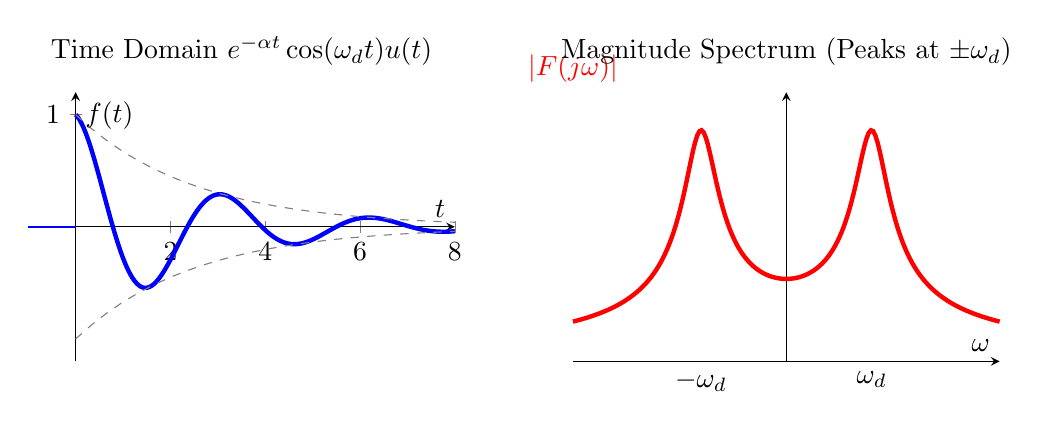
\begin{tikzpicture}
    \begin{groupplot}[
        group style={group size=2 by 1, horizontal sep=1.5cm},
        axis lines = middle,
        width = 7cm, height = 5cm,
        grid=none,
        xlabel = {$t$},
        ylabel = {$f(t)$}
    ]
        % Time Domain Damped Cosine
        \nextgroupplot[
            title = {Time Domain $e^{-\alpha t}\cos(\omega_d t)u(t)$},
            xmin = -1, xmax = 8,
            ymin = -1.2, ymax = 1.2,
            ytick = {1},
            yticklabels = {$1$}
        ]
        \addplot[ultra thick, blue, domain=0:8, samples=200] {exp(-0.4*x)*cos(deg(2*x))};
        \addplot[dashed, gray, domain=0:8] {exp(-0.4*x)};
        \addplot[dashed, gray, domain=0:8] {-exp(-0.4*x)};
        \draw[blue, thick] (-1,0) -- (0,0);

        % Frequency Domain Magnitude (Sketch)
        \nextgroupplot[
            title = {Magnitude Spectrum (Peaks at $\pm \omega_d$)},
            xlabel = {$\omega$},
            ylabel = {$|F(j\omega)|$},
            ylabel style={at={(axis description cs:0,1)},anchor=south, red},
            xmin = -5, xmax = 5,
            ymin = 0, ymax = 1.6,
            ytick = \empty,
            xtick = \empty,
            clip = false
        ]
        \addplot[ultra thick, red, domain=-5:5, samples=200] {0.5/sqrt(0.16 + (x-2)^2) + 0.5/sqrt(0.16 + (x+2)^2)};
        \node[anchor=north] at (axis cs:2, 0) {$\omega_d$};
        \node[anchor=north] at (axis cs:-2, 0) {$-\omega_d$};

    \end{groupplot}
\end{tikzpicture}
\end{document}
